
\documentclass{article}

% if you need to pass options to natbib, use, e.g.:
% \PassOptionsToPackage{numbers, compress}{natbib}
% before loading nips_2016
%
% to avoid loading the natbib package, add option nonatbib:
% \usepackage[nonatbib]{nips_2016}

% \usepackage{nips_2016}

% to compile a camera-ready version, add the [final] option, e.g.:
\usepackage[final]{nips_2016}
\usepackage[utf8]{inputenc} % allow utf-8 input
\usepackage[T1]{fontenc}    % use 8-bit T1 fonts
\usepackage{hyperref}       % hyperlinks
\usepackage{url}            % simple URL typesetting
\usepackage{booktabs}       % professional-quality tables
\usepackage{amsfonts}       % blackboard math symbols
\usepackage{nicefrac}       % compact symbols for 1/2, etc.
\usepackage{microtype}      % microtypography
\usepackage{amsmath}
\usepackage{cleveref}
\usepackage{algorithm}% http://ctan.org/pkg/algorithms
% \usepackage{algorithmic}
\usepackage{algpseudocode}
\usepackage{amsmath}
\usepackage{amssymb}
% \usepackage{amsfonts}
\usepackage{graphicx}
\usepackage{listings}
\usepackage{qtree}
\usepackage{pgf}
\usepackage{subfig}
\usepackage{tikz, calc}
\usepackage{natbib}
\newcommand{\vect}{\text{vec}}
\newcommand{\diag}{\text{diag}}
\newcommand{\rank}{\text{rank}}
\newcommand{\tr}{\text{tr}}
\newcommand{\prox}{\text{prox}}
\newcommand{\vecc}{\text{vec}}
\algnewcommand\algorithmicinput{\textbf{Input:}}
\algnewcommand\INPUT{\item[\algorithmicinput]}
\algnewcommand\algorithmicoutput{\textbf{Output:}}
\algnewcommand\OUTPUT{\item[\algorithmicoutput]}
\title{Algorithms Associated with Factorization Machines}

% The \author macro works with any number of authors. There are two
% commands used to separate the names and addresses of multiple
% authors: \And and \AND.
%
% Using \And between authors leaves it to LaTeX to determine where to
% break the lines. Using \AND forces a line break at that point. So,
% if LaTeX puts 3 of 4 authors names on the first line, and the last
% on the second line, try using \AND instead of \And before the third
% author name.

\author{
  Yanyu Liang \quad Xupeng Tong \quad Xin Lu\\
  % Computational Biology Department\\
  % Carnegie Mellon University\\
  % Pittsburgh, PA 15213 \\
  % \texttt{yanyul@andrew.cmu.edu} \\
  % \And
  %  \\
  Computational Biology Department\\
  Carnegie Mellon University\\
  Pittsburgh, PA 15213 \\
  \texttt{\{yanyul,xtong,xlu2\}@andrew.cmu.edu} \\
  % \AND
  %  \\
  % Computational Biology Department\\
  % Carnegie Mellon University\\
  % Pittsburgh, PA 15213 \\
  % \texttt{xlu2@andrew.cmu.edu} \\
  %% \And
  %% Coauthor \\
  %% Affiliation \\
  %% Address \\
  %% \texttt{email} \\
  %% \And
  %% Coauthor \\
  %% Affiliation \\
  %% Address \\
  %% \texttt{email} \\
}

\begin{document}
% \nipsfinalcopy is no longer used

\maketitle

\begin{abstract}
  Factorization machines (FMs) is widely used in recommendation system and it models the interaction between features by projecting $x \in \mathbb{R}^{p}$ onto the column space of $V \in \mathbb{R}^{k \times p}$. With the fact that $k < p$, it overcomes overfitting by limiting the second-order interaction term to be a low rank matrix. Based on FMs, researchers have proposed two extensions: i) convex FMs; ii) generalized FMs. In this report, we proposed and implemented two-block coordinate descent method with proximal gradient as subroutine for solving the original form of convex FMs proposed by \cite{convexFM_paper}. Beyond that, we extended convex FMs by introducing an element-wise sparsity constraint on interaction matrix, and we proposed and implemented an ADMM approach to solve this problem. Finally, we did empirical analysis on the performance of the algorithm proposed by \cite{generalizedFM_paper} for solving generalized FMs.
\end{abstract}

\section{Background}


Factorization machines were proposed in \cite{FM_paper}, which has been used heavily in recommendation system. FMs introduce higher-order term to model interaction between features which works reasonably well in recommendation system context, where input data is sparse but contains some low-dimensional structure, e.g. user tends to rate more movies in a specific genre. For $x \in \mathbb{R}^p$, FMs define $f: \mathbb{R}^p \rightarrow \mathbb{R}$ using the formalization shown in \cref{eq:original}. 
\begin{align}
  \hat{y} &= w_0 + w^T x + \sum_{i = 1}^p\sum_{j = i + 1}^p v_i^T v_j x_i x_j \label{eq:original} \\
  \hat{y} &= w_0 + w^T x + x^T W x \label{eq:reformal}
\end{align}
, where $v_i$ is k-by-1 vector and intuitively every feature is mapped to a $\mathbb{R}^k$ space where the inner product between two vectors describes the strength of interaction between two features. Here, FMs has a potential drawback, which is that FMs is nonconvex in $V$ and may be stuck at local optimum. From another perspective, if we let $V = (v_1, v_2, ..., v_p)$, then $\sum_{i = 1}^p\sum_{j = i + 1}^p v_i^T v_j x_i x_j = x^T V V^T x - x^T \diag(V V^T) x = x^T (V V^T -  \diag(V V^T))  x = x^T W x$. If we model $x_i^2$ term as well, $W$ is equivalent to $VV^T$ and $\rank(W) = k$. Therefore, we can think of FMs as a linear model with second-order term where coefficients of second-order term are regularized by a low rank constraint (see \cref{eq:reformal}). With this idea, \cite{convexFM_paper} proposed a convex formulation of FMs (cFMs), where instead of using $V$ they used $W$ directly to formalize the problem, which leads the whole problem to be convex. To solve cFMs problem, they proposed a coordinate descent method where they iteratively optimize $w_0, w$ and $W$, and in updating $W$, they greedily added rank-1 matrix. Besides convex formulation, \cite{generalizedFM_paper} reformulated the FMs by removing the implicit constraint that $W$ should be symmetric, positive semi-definite, and $W$ has zeros in diagonal entries, and they called the new model as generalized FMs (gFMS). Namely, they replace $W = V^TV$ with $U^TV$. To solve gFMs, they proposed a mini-batch algorithm which guarantees to converge with $O(\epsilon)$ reconstruction error when the sampling complexity is $O(k^3p \log(1/\epsilon))$. 


\section{Our work outline}

The goal of the project is to explore the optimization method for cFMs, and gFMs in regression setting with squared error loss as criteria (\cref{eq:criteria}),
\begin{align}
  f(w_0, w, W) &= \sum_{i = 1}^n (y^i - \hat{y}^i)^2 \label{eq:criteria}\\
  \text{, where} \quad \hat{y} &= w_0 + w^T x + x^T W x \quad\text{(cFMs)} \nonumber\\
  \hat{y} &= w_0 + w^T x + x^T U^TV x \quad\text{(gFMs)} \nonumber
\end{align}
In cFMs problem, we implemented a blockwise coordinate descent approach for solving the same objective (\cref{eq:criteria1}) as \cite{convexFM_paper} proposed. Beyond that, we introduced an additional regularizer $\|\vecc(W)\|_1$ to the original problem (see \cref{eq:criteria2}) and solved it using ADMM approach. 
\begin{align}
  L(w_0, w, W) &= f(w_0, w, W) + \lambda_1 \|W\|_{\tr} + \lambda_3 \|w\|_2^2 \label{eq:criteria1} \\
  L(w_0, w, W) &= f(w_0, w, W) + \lambda_1 \|W\|_{\tr} + \lambda_2 \|\vecc(W)\|_1 + \lambda_3 \|w\|_2^2 \label{eq:criteria2} 
\end{align}
For gFMs, we applied the algorithm proposed in \cite{generalizedFM_paper} and analyzed its performance empirically.

\section{Methods}

In this section, we describe the algorithms we used in details. \Cref{sec:cfm} introduces the proximal gradient descent for solving cFMs with trace norm constraint on $W$. \Cref{sec:admm} introduces the ADMM approach for solving cFMs with both trace norm and element-wise $l_1$ norm constraints.


\subsection{Solving cFMs by two-block coordinate descent} \label{sec:cfm}

To solve cFMs in the form of \cref{eq:criteria1}, we can re-form it in the following way:
\begin{equation}
\label{eq:eq5}
 \min_{w \in \mathbb{R}^{p}, W \in \mathbb{S}^{p \times p}} \;
\sum_{i = 1}^n 1/2(y_i-w^T x_i-x_i^T W x_i)^2 + \alpha /2 \|w\|_2^2 + \beta\|W\|_{\text{tr}}
\end{equation}
. To solve the problem, \cite{convexFM_paper} proposes a two-block descent algorithm, which separates the original problem into two sub-problems:
\begin{equation}
\label{eq:ridge}
 \min_{w \in \mathbb{R}^{d}} \;
\sum_{i = 1}^n 1/2(y_i-w^T x_i-\pi_i)^2 + \alpha /2 \|w\|_2^2,
\end{equation}
where $\pi_i=\langle W,x_i x_i^T\rangle$, and
\begin{equation}
\label{eq:proximal}
 \min_{W \in \mathbb{S}^{d*d}} \;
\sum_{i = 1}^n 1/2(y_i-w^T x_i-x_i^T W x_i)^2 + \beta\|W\|_{\text{tr}}
\end{equation}
Alternatively perform standard method on \cref{eq:ridge} and greedy coordinate descent on \cref{eq:proximal} until convergence will get optimal solution $w$ and $W$.
Similarly, we also perform the two-block descent algorithm. But the difference from \cite{convexFM_paper} is that, instead of greedy coordinate descent, here we solve \cref{eq:proximal} using proximal gradient descent. As for solving \cref{eq:ridge}, we consider it as solving a standard ridge regression problem.
We choose just perform gradient descent: let \cref{eq:ridge} be $f_1(w)$, then
$\nabla f_1(w)=-X'(y-diag(XZX')-Xw)+\alpha w$. So the gradient update is $w^+=w-t\nabla f_1(w)$. Thus, we get our gradient descent ridge solver with respect to $w$.
Then we consider solve \cref{eq:proximal} using proximal gradient descent. \cref{eq:proximal} can be written as $g(W)+h(W)$, where $g(W)=\sum_{i = 1}^n 1/2(y_i-w^T x_i-x_i^T W x_i)^2$ and
$h(W)=\beta\|W\|_{\text{tr}}$. Then we have
$$\nabla g(W)=-\sum_{i = 1}^n(y_i-w^T x_i-x_i^T W x_i)x_i x_i^T$$.
 
From what we know in class, for matrix completion problem,
$$\prox_t(W^{+})=S_{\beta t}(W^{+})=U\Sigma_{\beta t} V^T$$\\
where $W=U\Sigma V^T$ is a SVD, and $\Sigma_{\beta t}$ is diagonal matrix with $$(\Sigma_{\beta t})_{ii}=\max\{\Sigma_{ii}-\beta t,0\}$$
 
We then operate the backtracking line search on $g(W)$:
Define
$$G_t(W)=\left(W-\prox_t(W-t\nabla g(W))\right)/t$$
Then fix a parameter $0 <\beta < 1$. At each iteration, start with t = 1, and while
$$g(W-tG_t(W))>g(W)-t\nabla g(W)^T G_t(W)+\frac{t}{2}\|G_t(W)\|_F^2$$
shrink $t=\beta t$, else performs prox gradient update
$$\prox_t(W-t\nabla g(W))$$
Thus, we get our prox solver with respect to $W$.
 
Finally, perform the two-block descent algorithm: we iteratively perform the ridge solver and the prox solver until the optimal value meets our accuracy requirement.


\subsection{Solving sparse cFMs by ADMM} \label{sec:admm}

Recall that the objective \cref{eq:criteria2} has two nonsmooth terms in $W$, therefore the proximal gradient descent is not trivially applicable. However, by introducing an auxiliary $Z$ to replace one of the $W$ in the nonsmooth terms and adding another equality constraint $W - Z = 0$, the problem can be solved using ADMM. To minimize the number of calls for trace norm proximal opterator (it requires SVD which is computationally expensive), we chose to replace $\|W\|_{\tr}$ as $\|Z\|_{\tr}$, and then the augmented Lagrangian multiplier is:
\begin{align}
  \mathcal{L}(w_0, w, W, Z, u) &= f(w_0, w, W) + \lambda_1 \|Z\|_{\tr} + \lambda_2 \|\vecc(W)\|_1 + \lambda_3 \|w\|_2^2 \nonumber\\
  &+ \langle W - Z, u \rangle + m\|W - Z\|_F^2 \nonumber
\end{align}
, where $u \in \mathbb{R}^{p \times p}$ is dual variable and $m$ is parameter of the augmented term. 

Then the ADMM iterations can be summarized as follow:
\begin{enumerate}
    \item Update $w_0, w, W$:
    \begin{align*}
        w_0^k, w^k, W^k &= \arg\min_{w0, w, W} f(w_0, w, W) + \lambda_2 \|\vecc(W)\|_1 + \lambda_3 \|w\|_2^2 \\
        &+ \frac{\rho}{2} \|W - Z^{k - 1} + u^{k - 1}\|_F^2
    \end{align*}
    \item Update $Z$:
    \begin{align*}
        Z^k = \arg\min_Z \lambda_1 \|Z\|_{\tr} + \frac{\rho}{2}\|W^k - Z + u^{k-1}\|_F^2
    \end{align*}
    \item Update $u$:
    \begin{align*}
        u^k = u^{k - 1} + W^k - Z^k
    \end{align*}
\end{enumerate}

The second step can be solved exactly using matrix soft-thresholding operator as described before. But there is no closed form solution for the first subproblem. To solve the first step numerically, we applied two strategies: i) proximal gradient descent on $w_0, w, W$; ii) blockwise coordinate descent on $w_0, w$ and $W$ respectively, namely:
\begin{align}
  w_0, w &= \arg\min_{w0, w} f(w_0, w, W) + \lambda_3 \|w\|_2^2 \label{eq:subw0w} \\
  W &= \arg\min_W f(w_0, w, W) + \lambda_2 \|\vecc(W)\|_1 + \frac{\rho}{2} \|W - Z + u\|_F^2 \label{eq:subW}
\end{align}
Furthermore, in the coordinate descent, we update $w_0, w$ using another coordinate descent which converges quickly. But for the update of $W$, as the problem size is much bigger, it converges more slowly. Therefore, we tried two approches here to solve the subproblem on updating $W$: a) proximal gradient descent; b) quasi-Newton method (OWL-QN\cite{andrew2007scalable}). Then the overall procedure is summarized in \Cref{algo:admm}.

\begin{algorithm} 
  \caption{ADMM for solving \cref{eq:criteria2}}
  \label{algo:admm}
  \begin{algorithmic}[1]
    \INPUT{$w_0^0, w^0, W^0, Z^0, u^0, \rho$, maxstep, tol}
    \OUTPUT{$w_0, w^k, W$}
    \For{$k = 1$ : maxstep}
      \While{forward error $>$ tol}
        \State update $w_0^k, w^k, W^k$ with proximal gradient descent / blockwise coordinate descent
      \EndWhile 
      \State $Z^k = \prox_{\tr, \frac{\lambda_1}{\rho}}(W^k + u^{k - 1})$
      \State $u^k = W^k - Z^k$
    \EndFor
  \end{algorithmic}
\end{algorithm}

\section{Results}

In this section, we show the results of our algorithms running on simulated data, where $p$ varies in $10, 30, 100, 500, 1000$.  We used four types of $W$: i) $W = V^TV$ (SYM); ii) $W = U^TV$ (ASYM); iii) sparse $W$ (SPARSE); iv) block diagonal $W$ (BLOCK) shown in \Cref{fig:designW}.

\begin{figure}[htbp]
  \centering
  \begin{minipage}{0.24\textwidth}
    \centering
    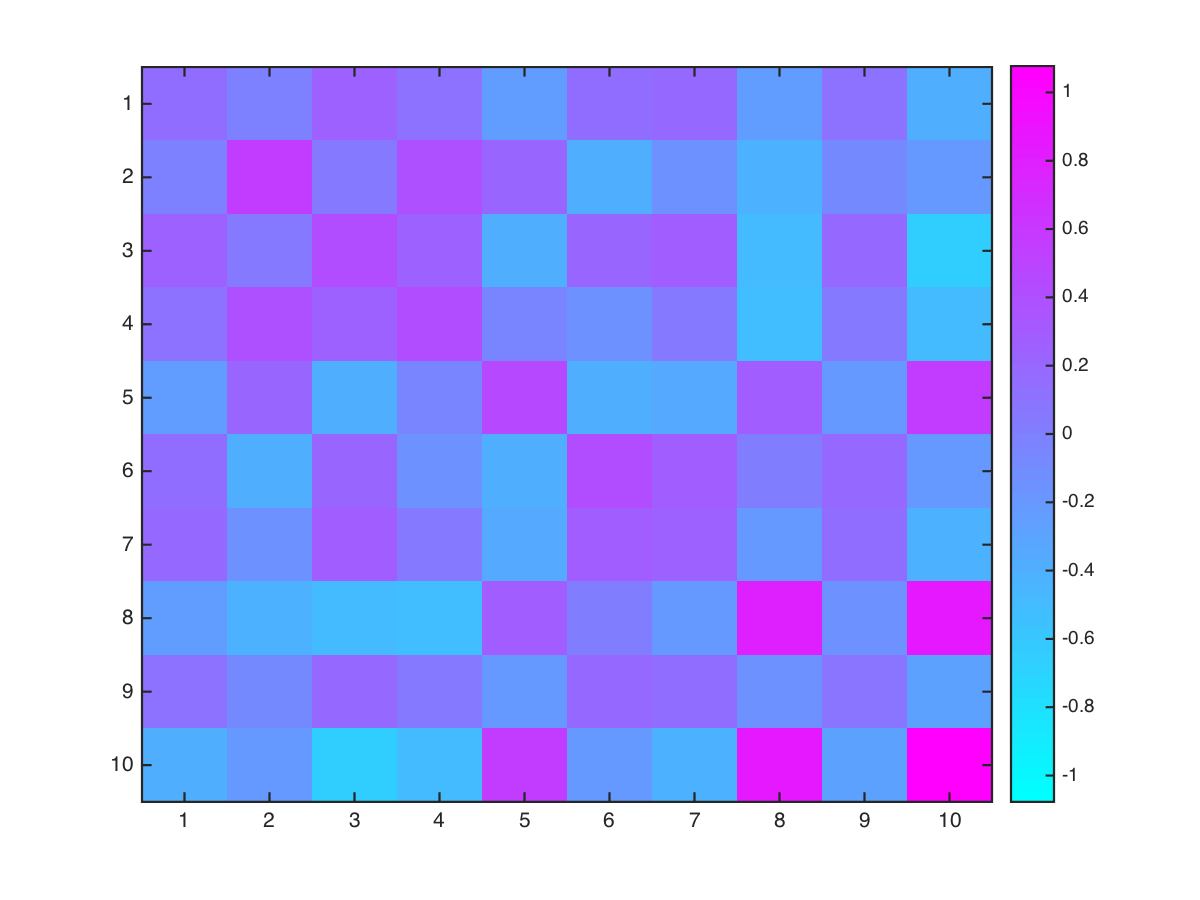
\includegraphics[width=1\textwidth]{../yanyu_code/plots/sym}
  \end{minipage}
  \hfill
  \begin{minipage}{0.24\textwidth}
    \centering
    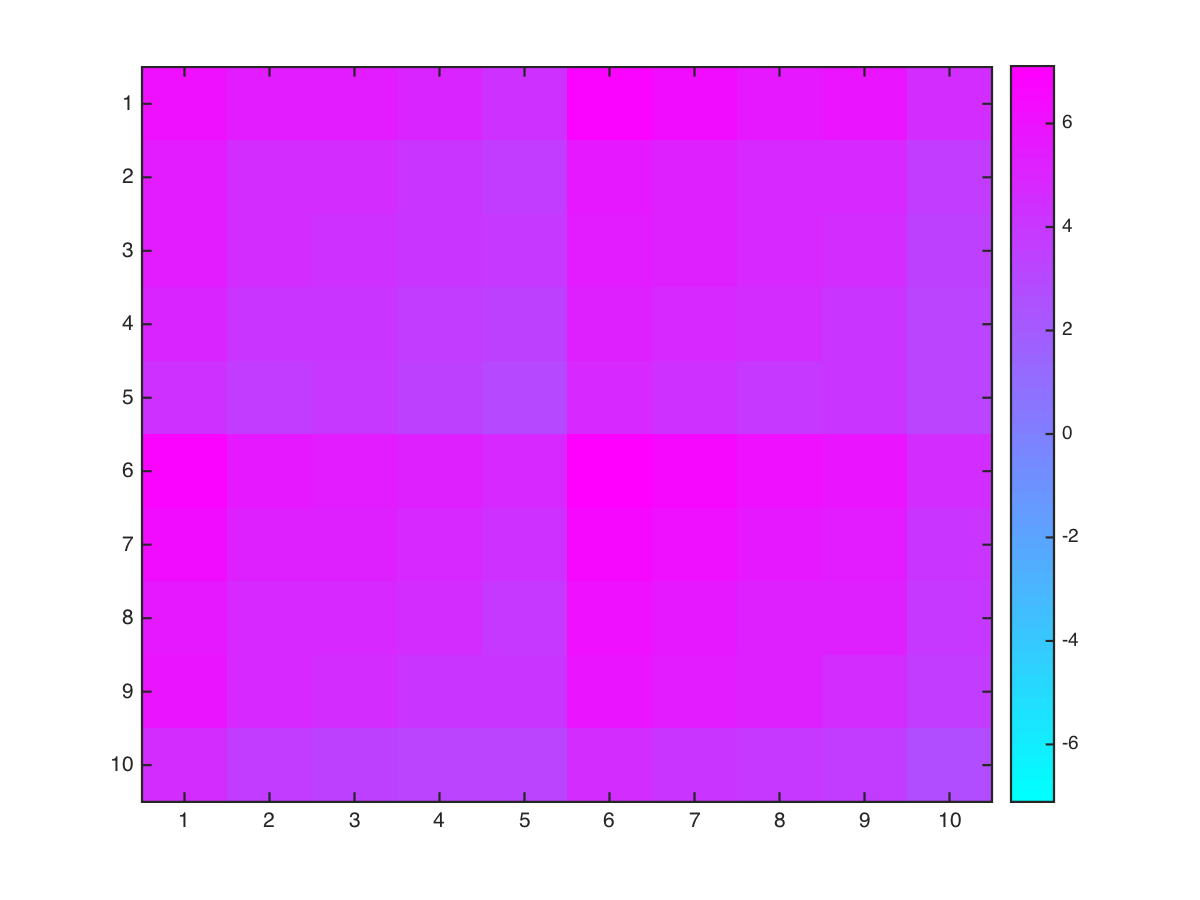
\includegraphics[width=1\textwidth]{../yanyu_code/plots/asym}
  \end{minipage}
  \hfill
  \begin{minipage}{0.24\textwidth}
    \centering
    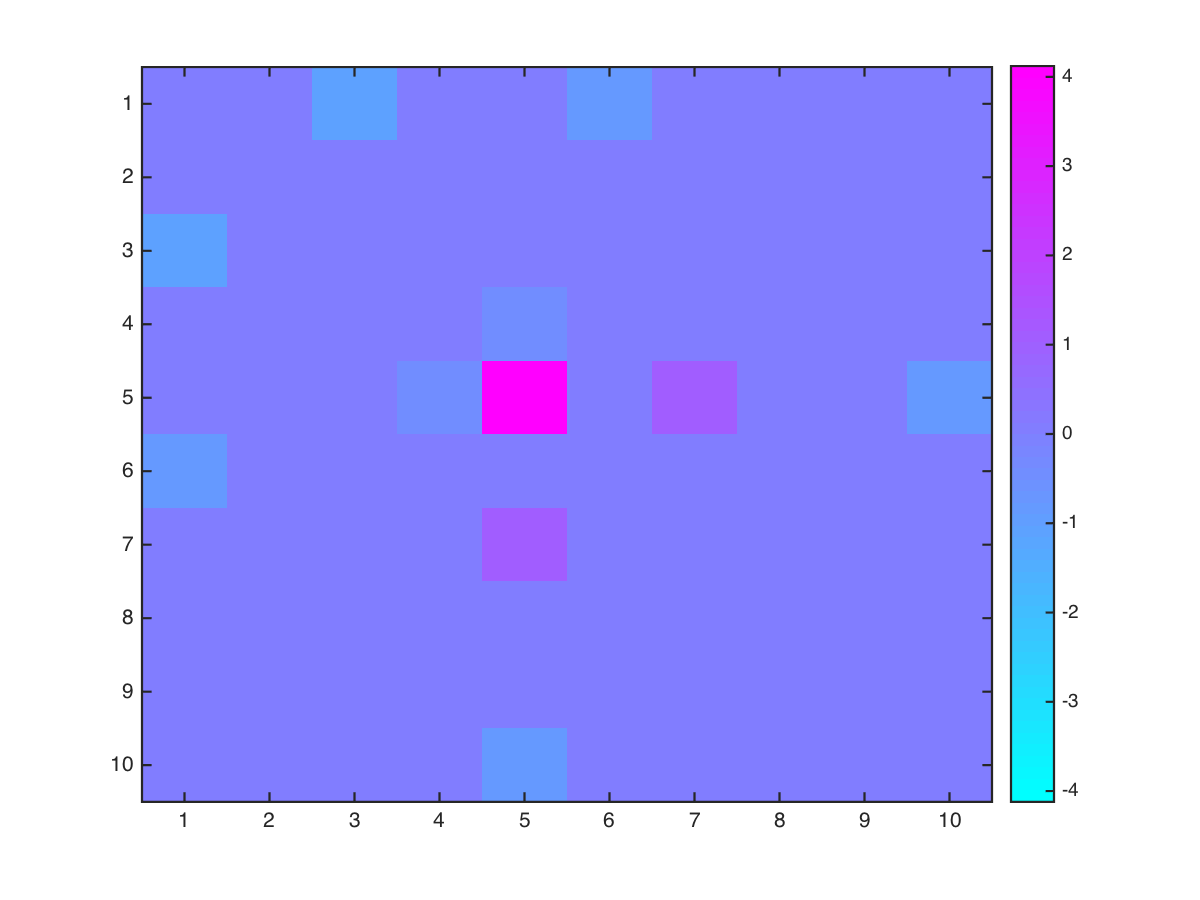
\includegraphics[width=1\textwidth]{../yanyu_code/plots/sparse}
  \end{minipage}
  \hfill
  \begin{minipage}{0.24\textwidth}
    \centering
    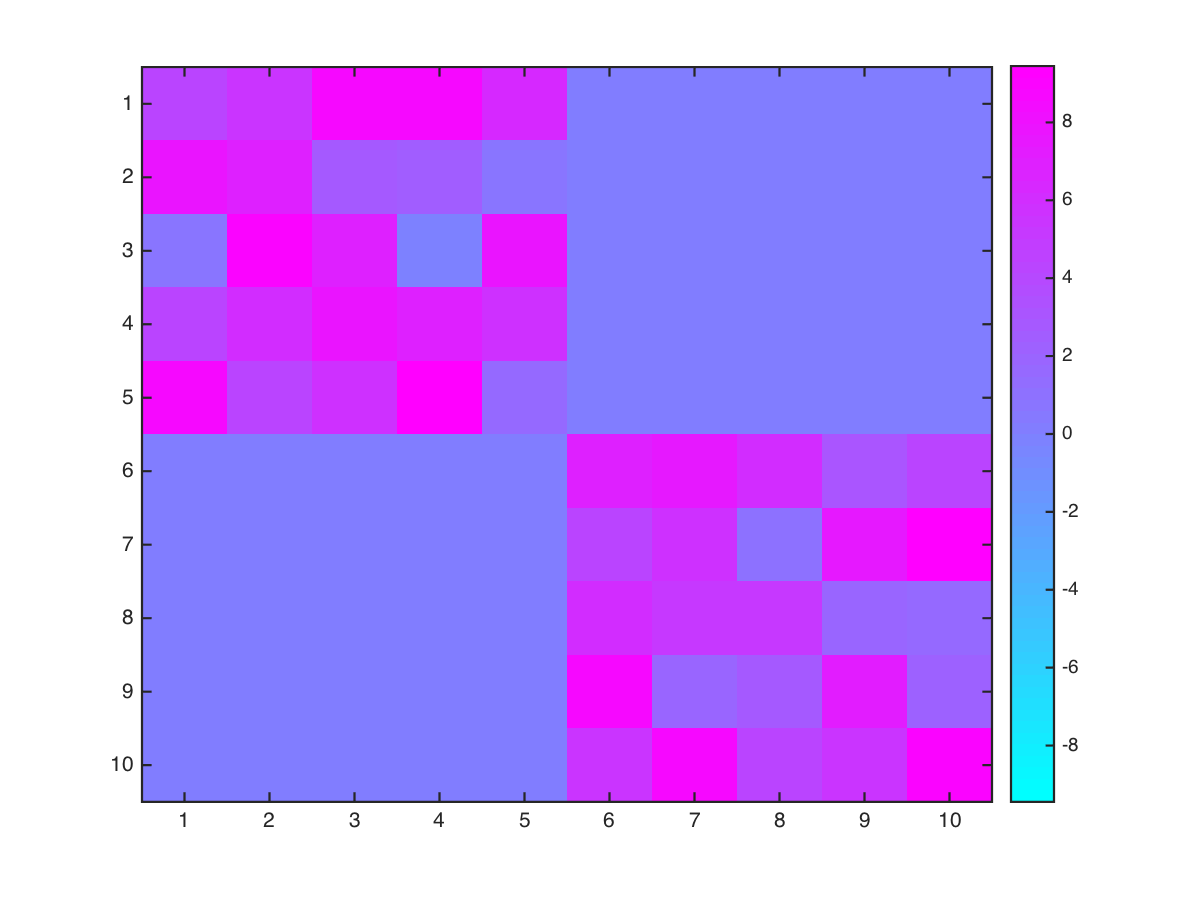
\includegraphics[width=1\textwidth]{../yanyu_code/plots/block}
  \end{minipage}
  \caption{$W$ matrix for four types of data (left to right: SYM, ASYM, SPARSE, BLOCK)}
  \label{fig:designW}
\end{figure}

\Cref{sec:result_cfm} presents the results in solving \cref{eq:criteria1} with method proposed in \Cref{sec:cfm}. \Cref{sec:result_scfm} presents the results in implementing the methods for \cref{eq:criteria2} proposed in \Cref{sec:admm}. Finally, we present the results of gFMs in \Cref{sec:result_gfm}.

\subsection{cFMs} \label{sec:result_cfm}

After several trials, based on our computing capacity, we found the proper feature dimension we are able to use for testing convexFMs is 10.

\Cref{fig:cfm_figs} shows the convergence rate of four data types. The order of the convergence rate is as follows: SYM$>$SPARSE$>$ASYM$\approx$BLOCK. Particularly, symmetric and sparse converge much more faster than asymmetric and block. Another interesting observation we want to point out is that, symmetric and sparse converge in a form we called "one stage convergence": objective value dramatically drop down at the first several iteration, then it almost don't quite drop much. As for, asymmetric and block, they perform like "two stage convergence", the first step is similar to one stage version, but there is another objective value drop down stage, but the speed is slower than the first one.
\begin{figure}[htbp]
  \centering
  \begin{minipage}{0.24\textwidth}
    \centering
    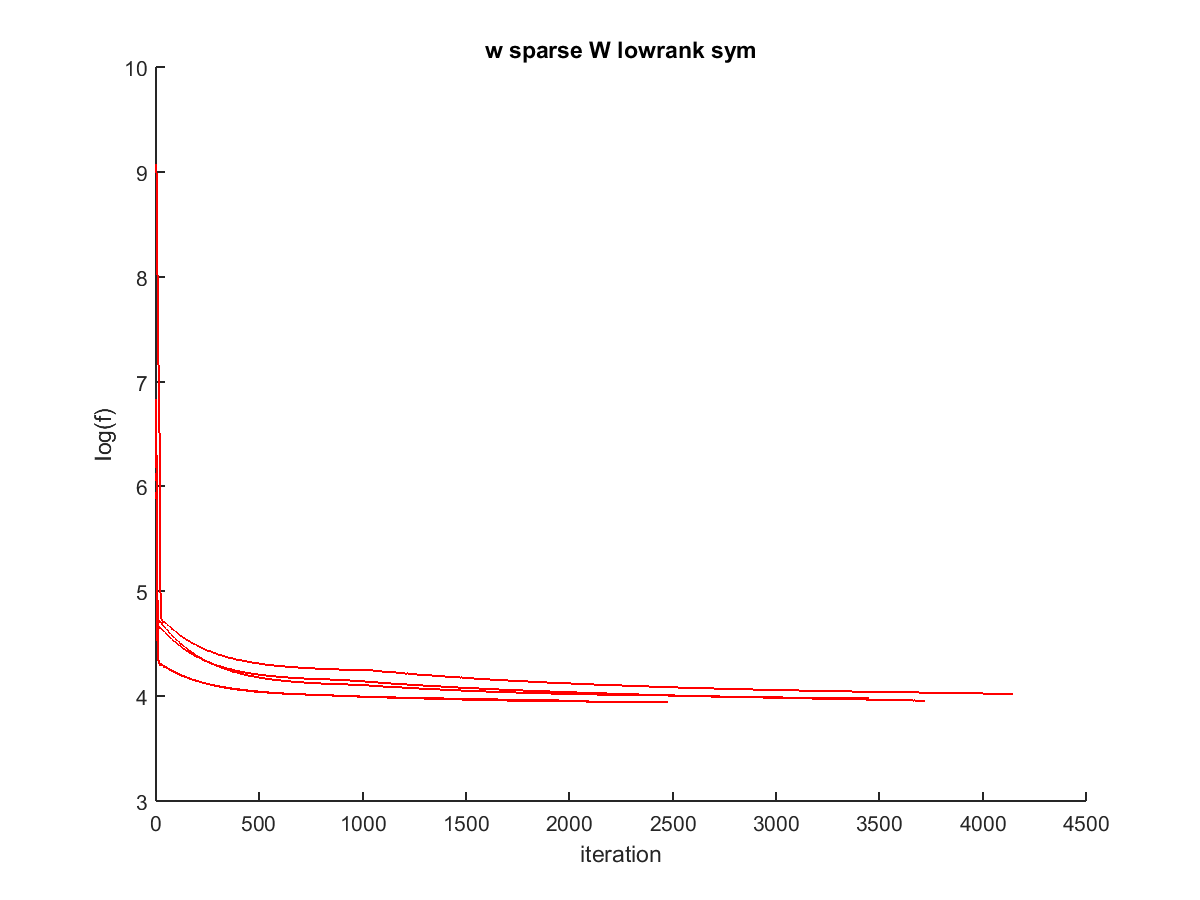
\includegraphics[width=1\textwidth]{images/xin_sym}
  \end{minipage}
  \hfill
  \begin{minipage}{0.24\textwidth}
    \centering
    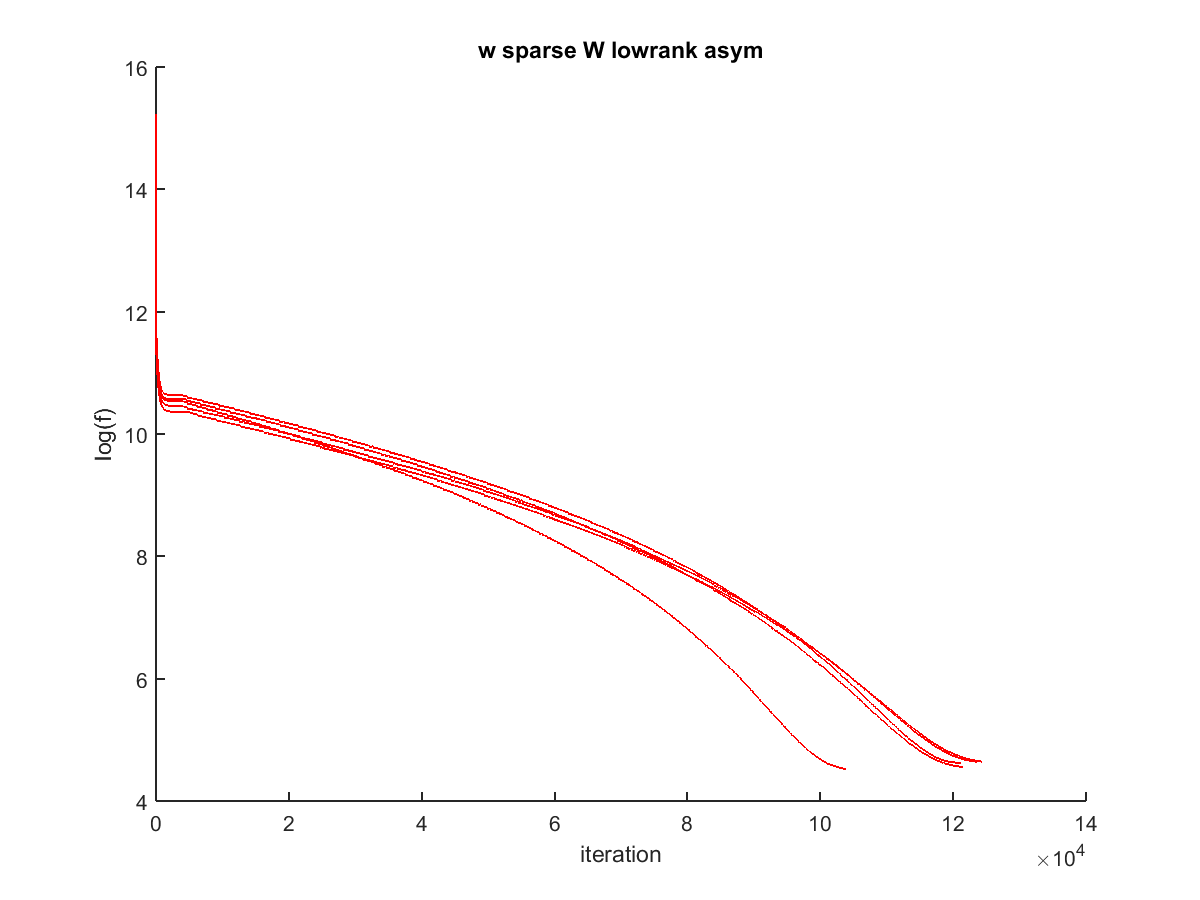
\includegraphics[width=1\textwidth]{images/xin_asym}
  \end{minipage}
  \hfill
  \begin{minipage}{0.24\textwidth}
    \centering
    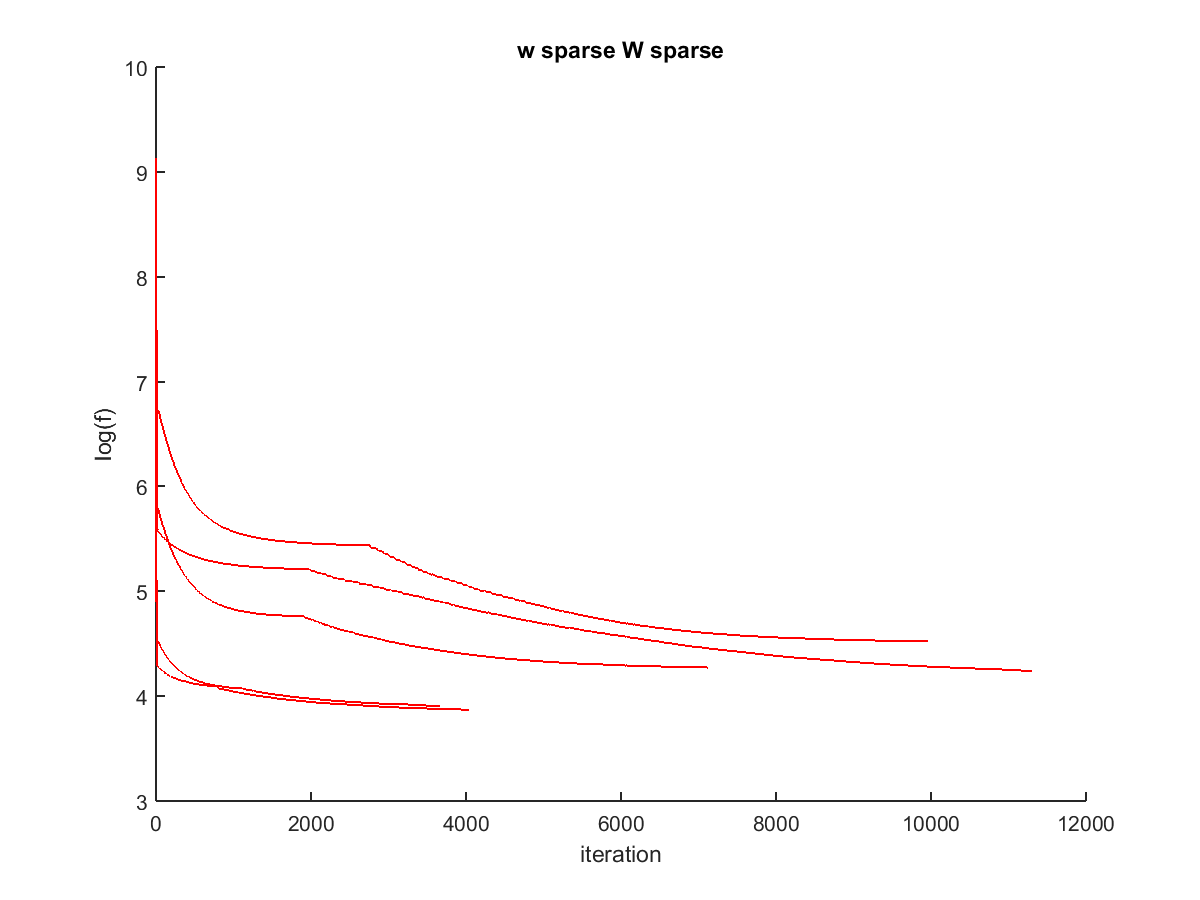
\includegraphics[width=1\textwidth]{images/xin_sparse}
  \end{minipage}
  \hfill
  \begin{minipage}{0.24\textwidth}
    \centering
    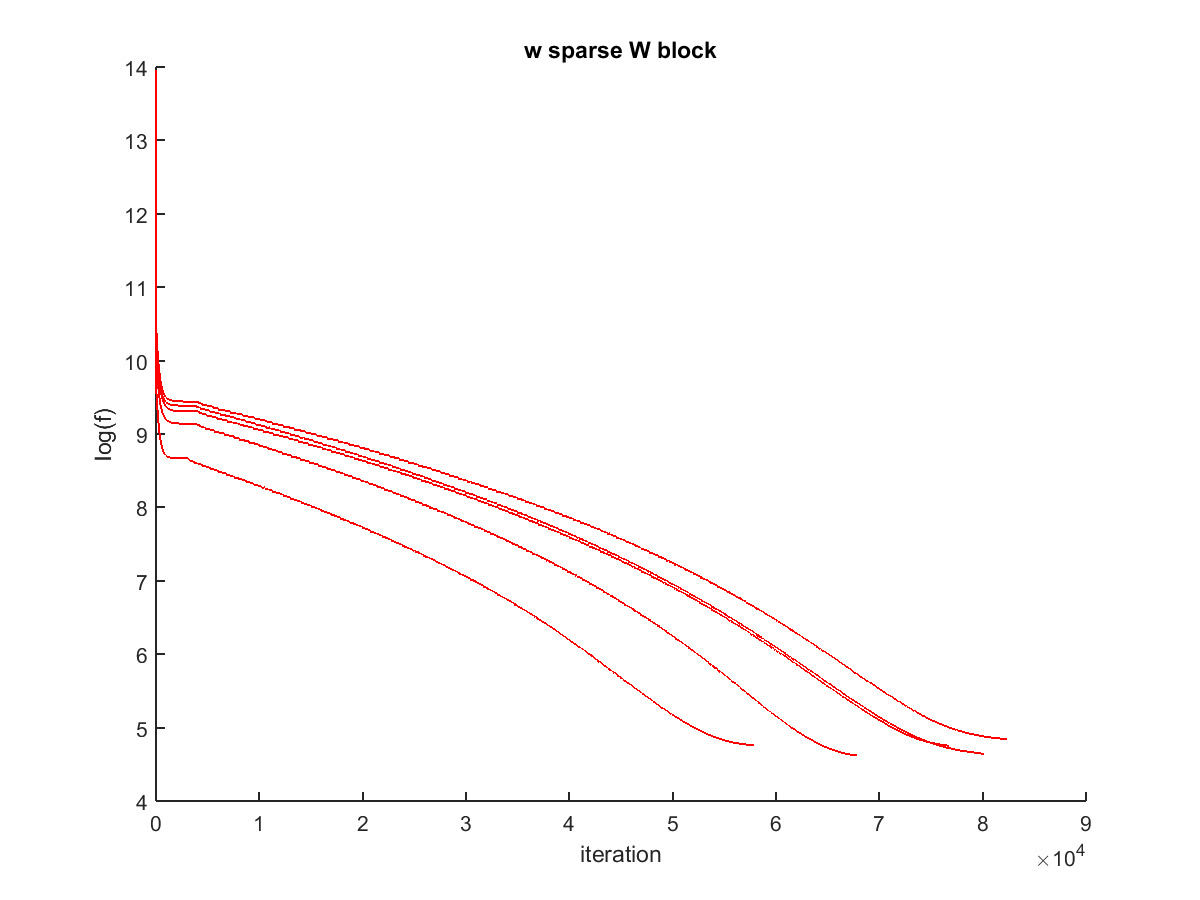
\includegraphics[width=1\textwidth]{images/xin_block}
  \end{minipage}
  \caption{cFMs: The convergences of two-block coordinate descent on four types of simulated data (left to right: SYM, ASYM, SPARSE, BLOCK)}
  \label{fig:cfm_figs}
\end{figure}

\subsection{sparse cFMs} \label{sec:result_scfm}

We first compare the performance of proximal gradient and quasi-Newton method on solving \cref{eq:subW}. The comparison of these two approaches in terms of convergence is shown in \Cref{fig:argminW_curve}. 
\begin{figure}[htbp]
  \centering
  \begin{minipage}{0.24\textwidth}
    \centering
    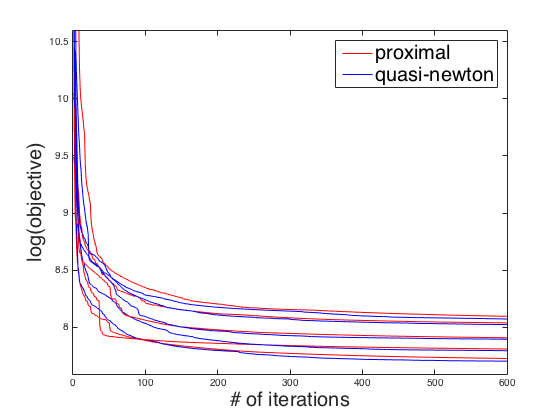
\includegraphics[width=1\textwidth]{../yanyu_code/plots/sym_p30}
  \end{minipage}
  \hfill
  \begin{minipage}{0.24\textwidth}
    \centering
    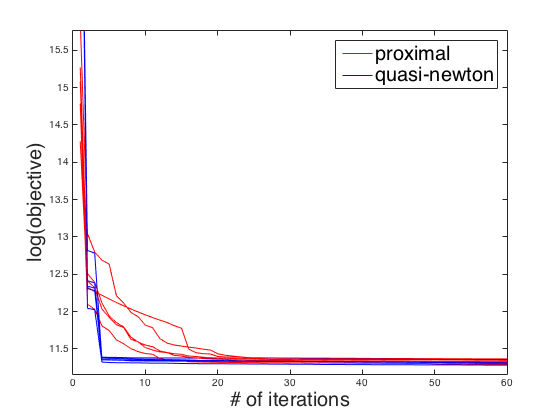
\includegraphics[width=1\textwidth]{../yanyu_code/plots/asym_p30}
  \end{minipage}
  \hfill
  \begin{minipage}{0.24\textwidth}
    \centering
    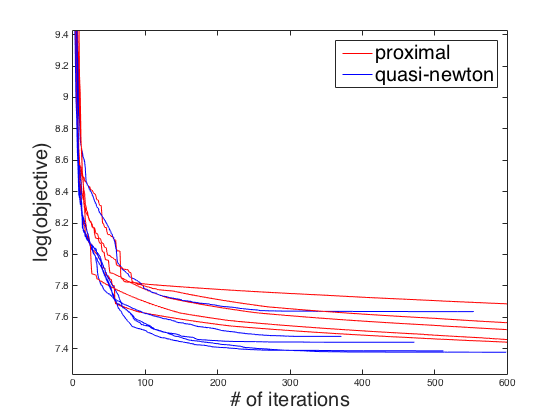
\includegraphics[width=1\textwidth]{../yanyu_code/plots/sparse_p30}
  \end{minipage}
  \hfill
  \begin{minipage}{0.24\textwidth}
    \centering
    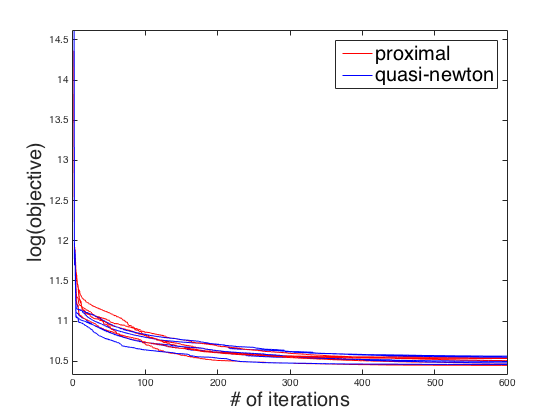
\includegraphics[width=1\textwidth]{../yanyu_code/plots/block_p30}
  \end{minipage}
  \caption{sparse cFMs (solve \cref{eq:subW}): The convergences of the two algorithms on four types of simulated data (left to right: SYM, ASYM, SPARSE, BLOCK)}
  \label{fig:argminW_curve}
\end{figure}
From the results we can see, Quasi-Newton is almost always outperforms first-order method in the sense that it can achieve the same results with fewer iterations, but the performance also depends on the property of the data. Furthermore, from the convergence curve we can see, if we stop the algorithm early, in SYM and BLOCK data, Quasi-Newton gives roughly the same result as proximal. Such results may result from the fact that in these data, the initial point is fairly far from the true optimizer.

Then we compared the performance of the following three algorithms in solving the first step in ADMM: i) proximal gradient descend on $w_0, w, W$ as a whole (referred as proximal); ii) block-wise coordinate descent with proximal gradient descent for $W$ and coordinate descent for $w_0, w$ as inner loops (referred as coord-quasiNewton); iii) block-wise coordinate descent with OWL-QN update for $W$ and coordinate descent for $w_0, w$ as inner loops (referred as coord-proximal). Their performances were tested on the same data sets, and the convergence curves are shown in \Cref{fig:argminw0wW_curve}. The percentages of $W$ updates in the coordinate decent methods are shown in \Cref{fig:argminw0wW_ratio}. 
\begin{figure}[htbp]
  \centering
  \begin{minipage}{0.24\textwidth}
    \centering
    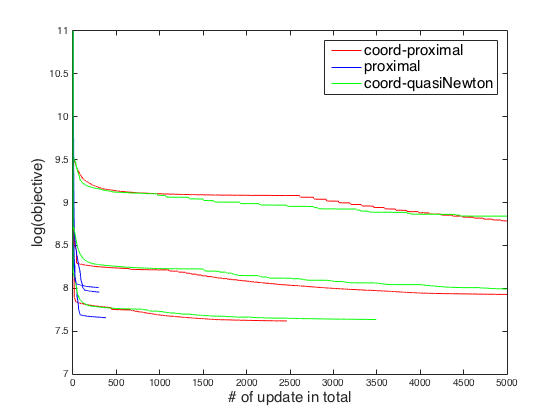
\includegraphics[width=1\textwidth]{../yanyu_code/plots/sym_w0wW_curve_p30}
  \end{minipage}
  \hfill
  \begin{minipage}{0.24\textwidth}
    \centering
    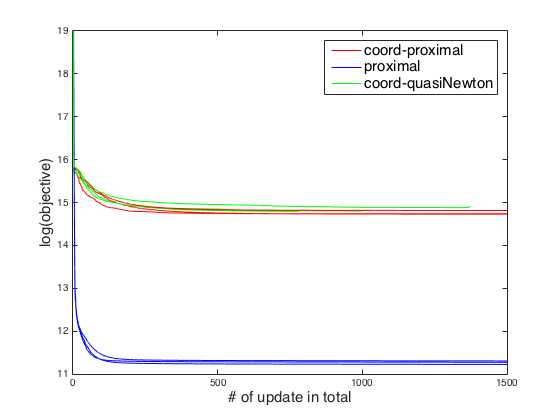
\includegraphics[width=1\textwidth]{../yanyu_code/plots/asym_w0wW_curve_p30}
  \end{minipage}
  \hfill
  \begin{minipage}{0.24\textwidth}
    \centering
    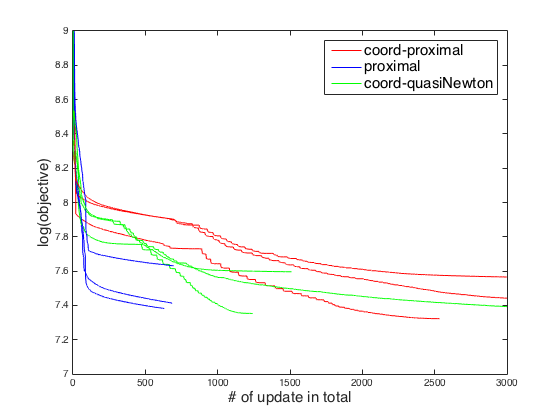
\includegraphics[width=1\textwidth]{../yanyu_code/plots/sparse_w0wW_curve_p30}
  \end{minipage}
  \hfill
  \begin{minipage}{0.24\textwidth}
    \centering
    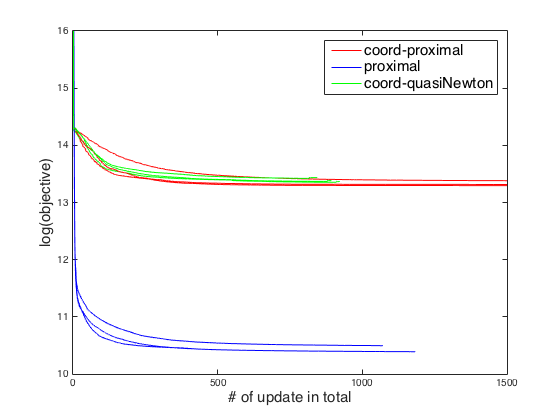
\includegraphics[width=1\textwidth]{../yanyu_code/plots/block_w0wW_curve_p30}
  \end{minipage}
  \caption{sparse cFMs (solve ADMM step1): The convergences of the three algorithms on four types of simulated data (left to right: SYM, ASYM, SPARSE, BLOCK)}
  \label{fig:argminw0wW_curve}
\end{figure}
\begin{figure}[htbp]
  \centering
  \begin{minipage}{0.24\textwidth}
    \centering
    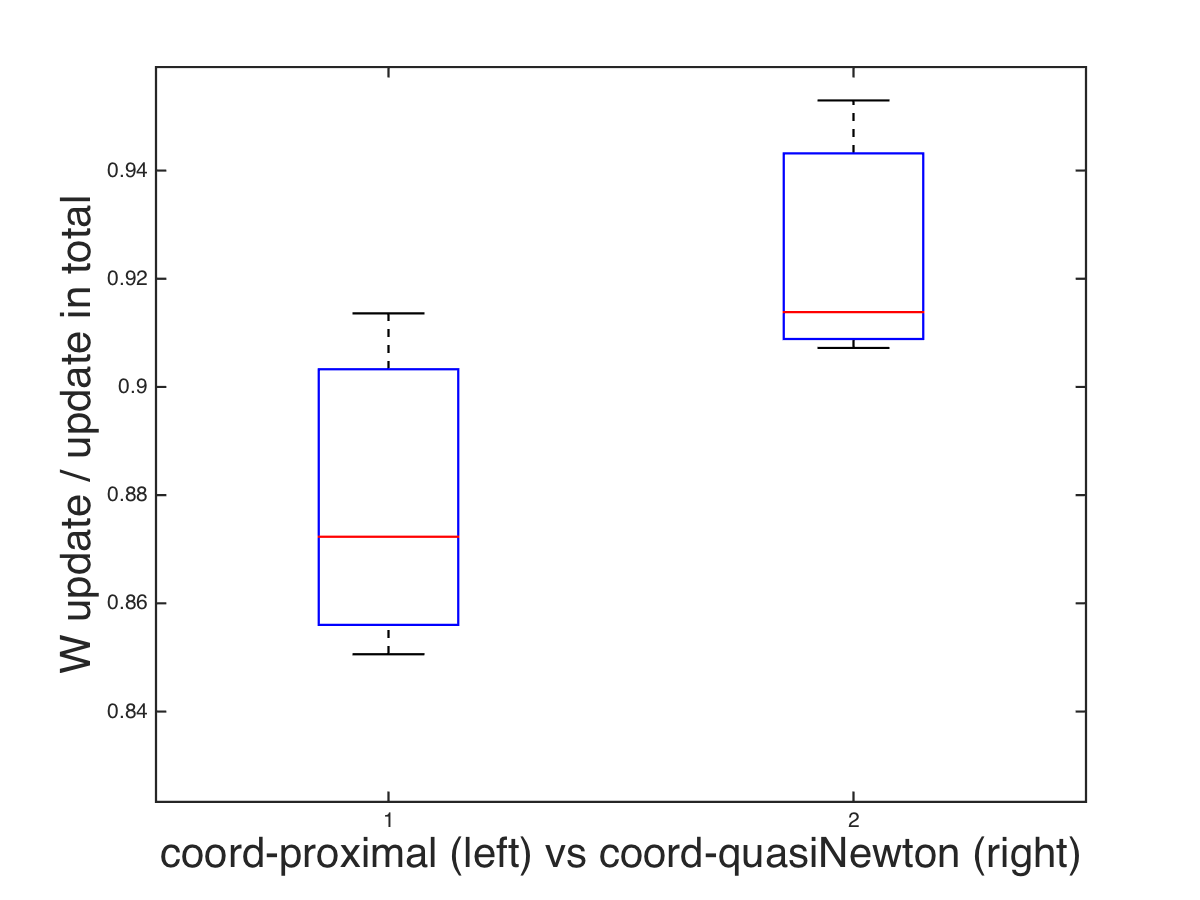
\includegraphics[width=1\textwidth]{../yanyu_code/plots/sym_w0wW_box_p30}
  \end{minipage}
  \hfill
  \begin{minipage}{0.24\textwidth}
    \centering
    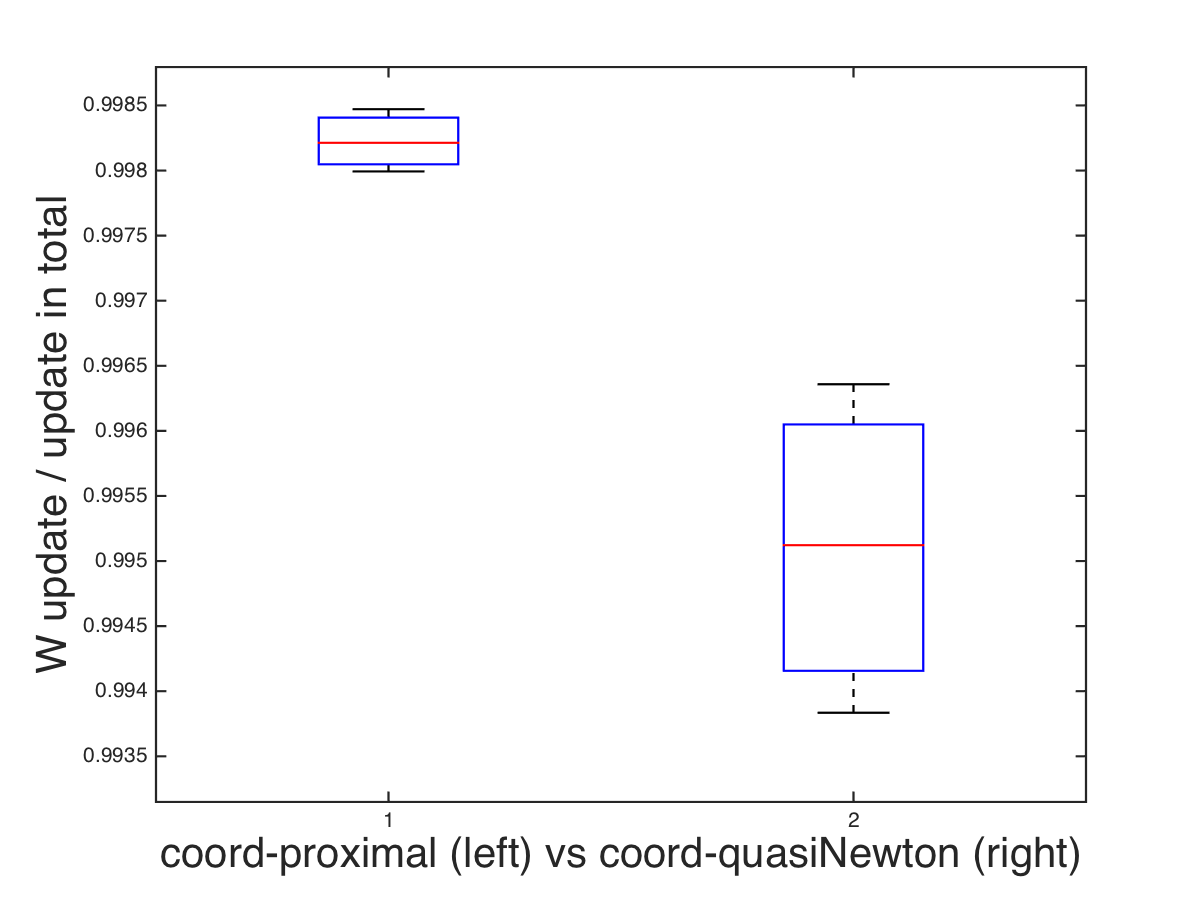
\includegraphics[width=1\textwidth]{../yanyu_code/plots/asym_w0wW_box_p30}
  \end{minipage}
  \hfill
  \begin{minipage}{0.24\textwidth}
    \centering
    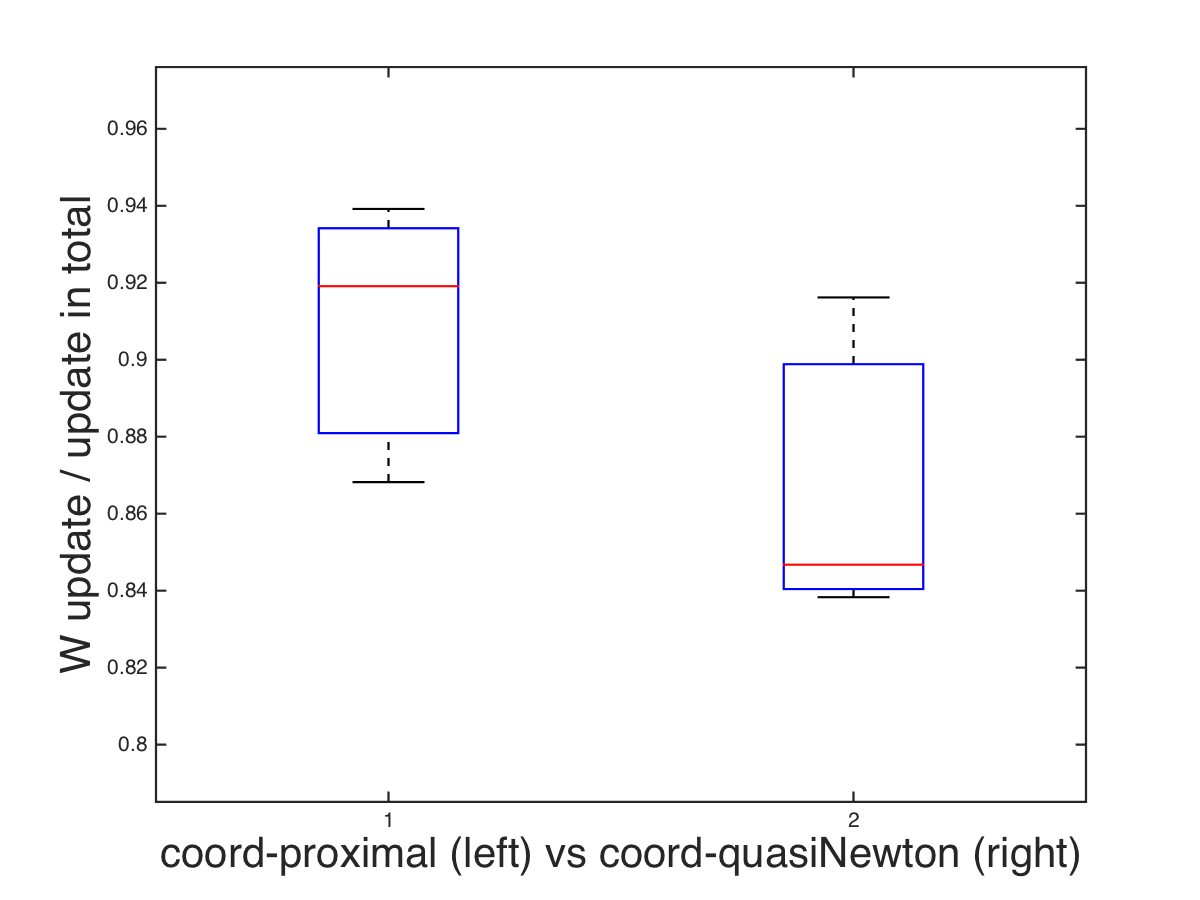
\includegraphics[width=1\textwidth]{../yanyu_code/plots/sparse_w0wW_box_p30}
  \end{minipage}
  \hfill
  \begin{minipage}{0.24\textwidth}
    \centering
    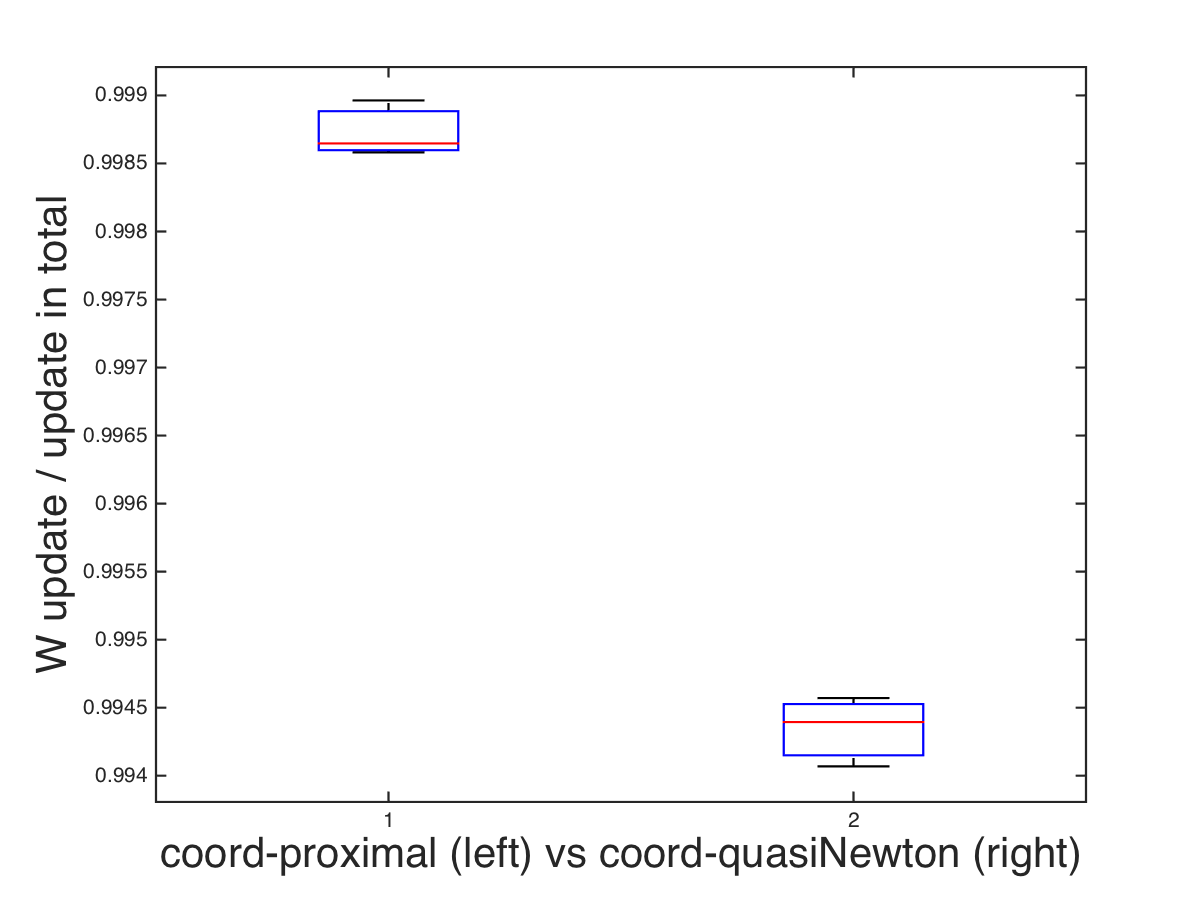
\includegraphics[width=1\textwidth]{../yanyu_code/plots/block_w0wW_box_p30}
  \end{minipage}
  \caption{sparse cFMs (solve ADMM step1): The percentage of $W$ updates in total updates for updating $w0, w, W$ in blockwise coordinate descent algorithms (left to right: SYM, ASYM, SPARSE, BLOCK)}
  \label{fig:argminw0wW_ratio}
\end{figure}
From the results we can see, solving \cref{eq:subW} used most of the updates, and it is reasonable since \cref{eq:subW} is a much bigger problem comparing to solving \cref{eq:subw0w}. Furthermore, proximal seems to be the most efficient algorithm in this problem. It converges quickly and always stops somewhere close to the optimum, whereas the blockwise coordinate descent may not converge to the right answer. The reason why coordinate descent algorithm get stuck at some point may result from the fact that inner problem is not solved inexactly. Moreover, coord-quasiNewton works than coord-proximal, which is consistent with the previous results. 

By applying the above three approaches as a subroutine in ADMM, the performance of the ADMM is shown in \Cref{fig:admm}. The feasibility (element-wise average of $\|W - Z\|_F^2$) is shown in \Cref{fig:feas}.
\begin{figure}[ht!]
  \centering
  \begin{minipage}{0.45\textwidth}
    \centering
    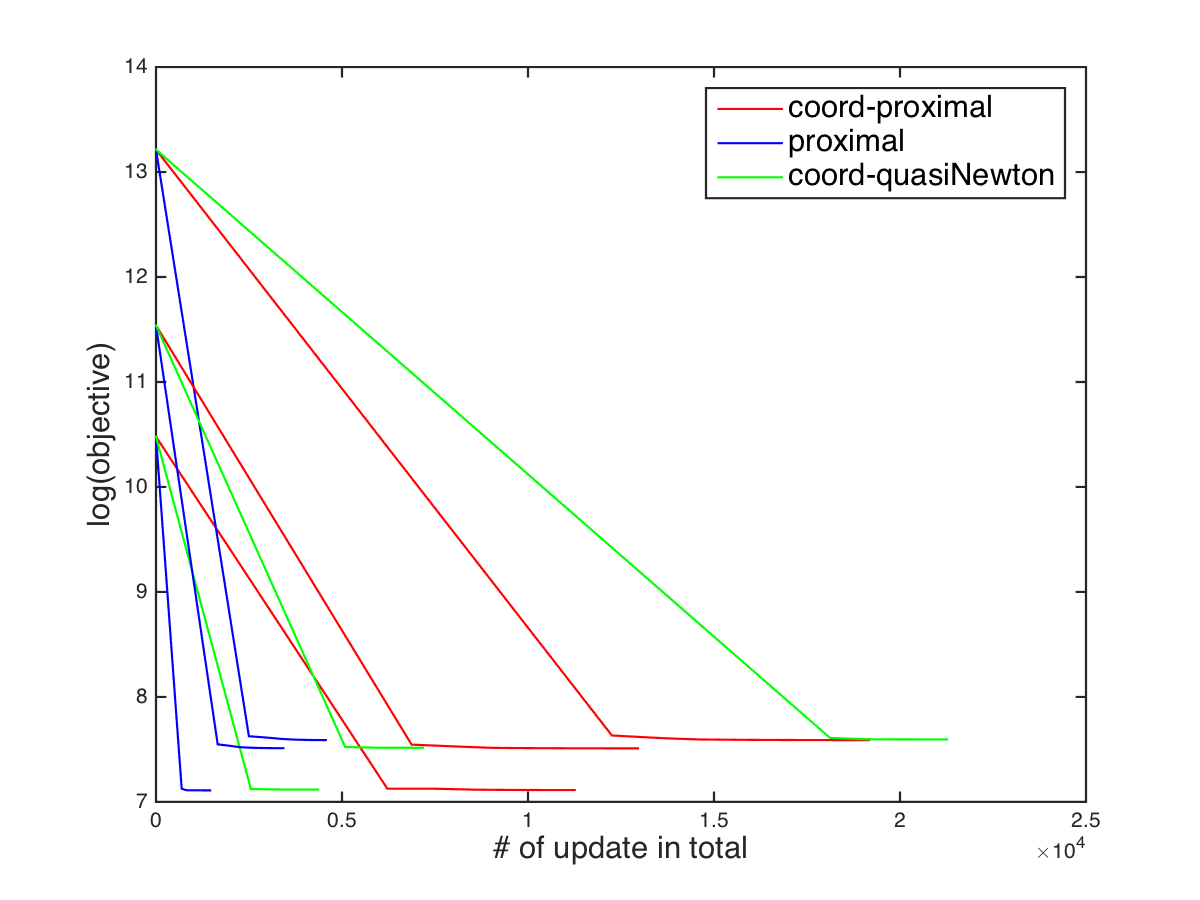
\includegraphics[width=.7\textwidth]{../yanyu_code/plots/sym_ADMM_obj_p30}
  \end{minipage}
  \hfill
  \begin{minipage}{0.45\textwidth}
    \centering
    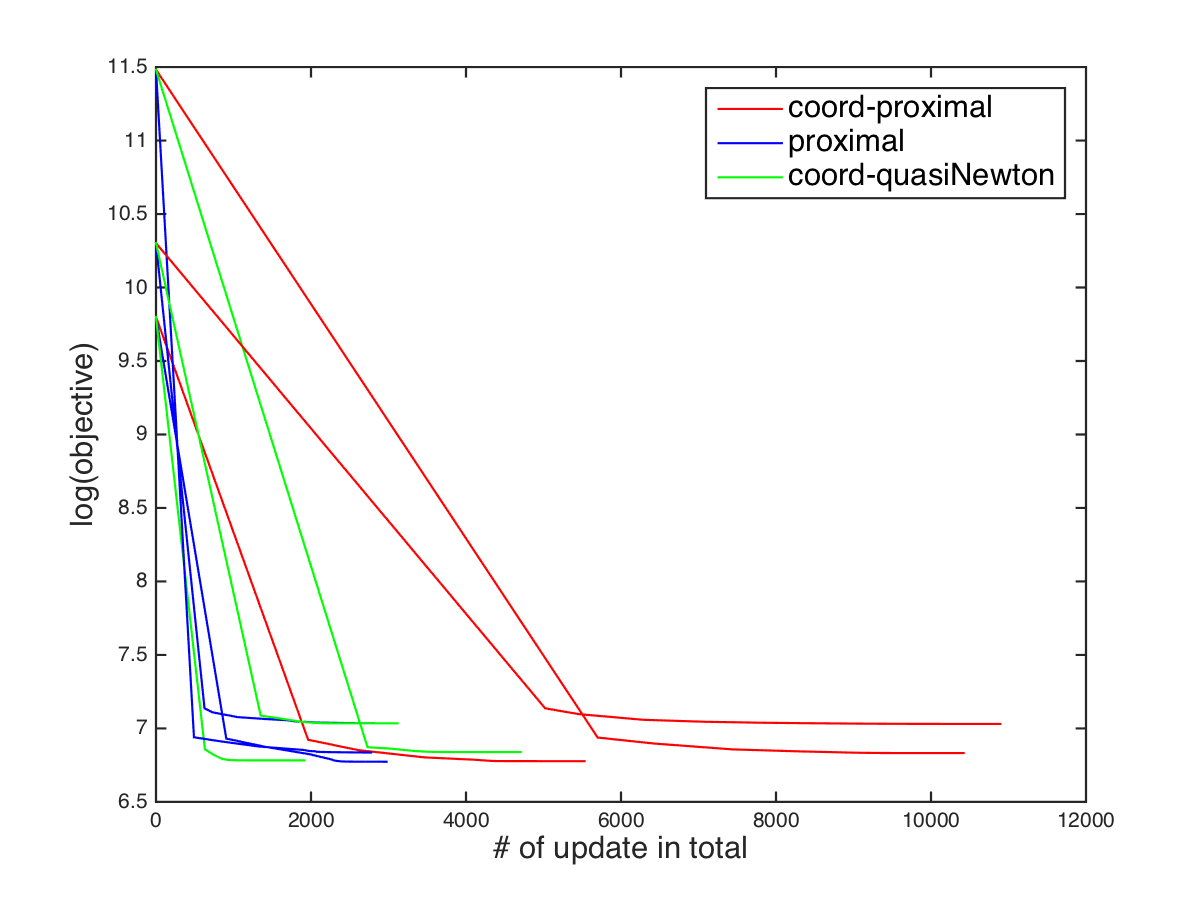
\includegraphics[width=.7\textwidth]{../yanyu_code/plots/sparse_ADMM_obj_p30}
  \end{minipage}
  \caption{sparse cFMs (ADMM): The convergences of three ADMMs on four types of simulated data (left to right: SYM, SPARSE)}
  \label{fig:admm}
\end{figure}
\begin{figure}[ht!]
  \centering
  \begin{minipage}{0.45\textwidth}
    \centering
    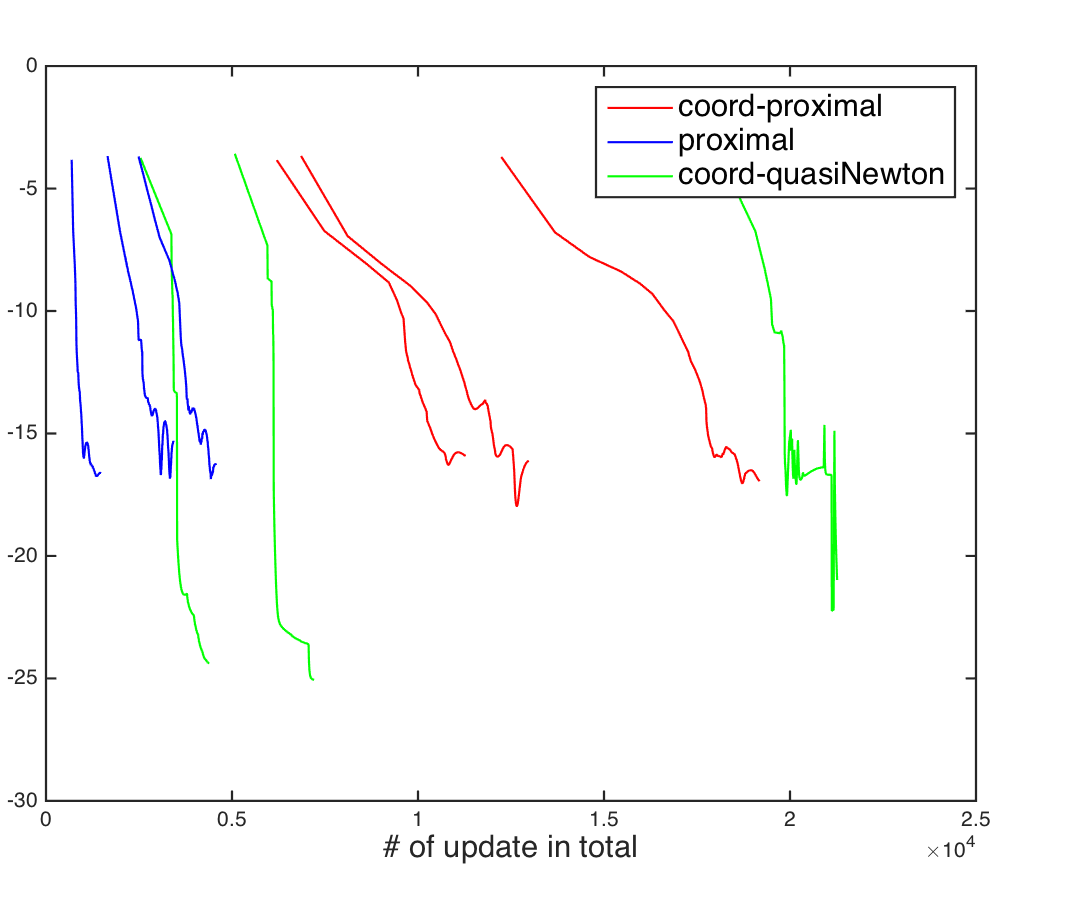
\includegraphics[width=.65\textwidth]{../yanyu_code/plots/sym_ADMM_feasibility_p30}
  \end{minipage}
  \hfill
  \begin{minipage}{0.45\textwidth}
    \centering
    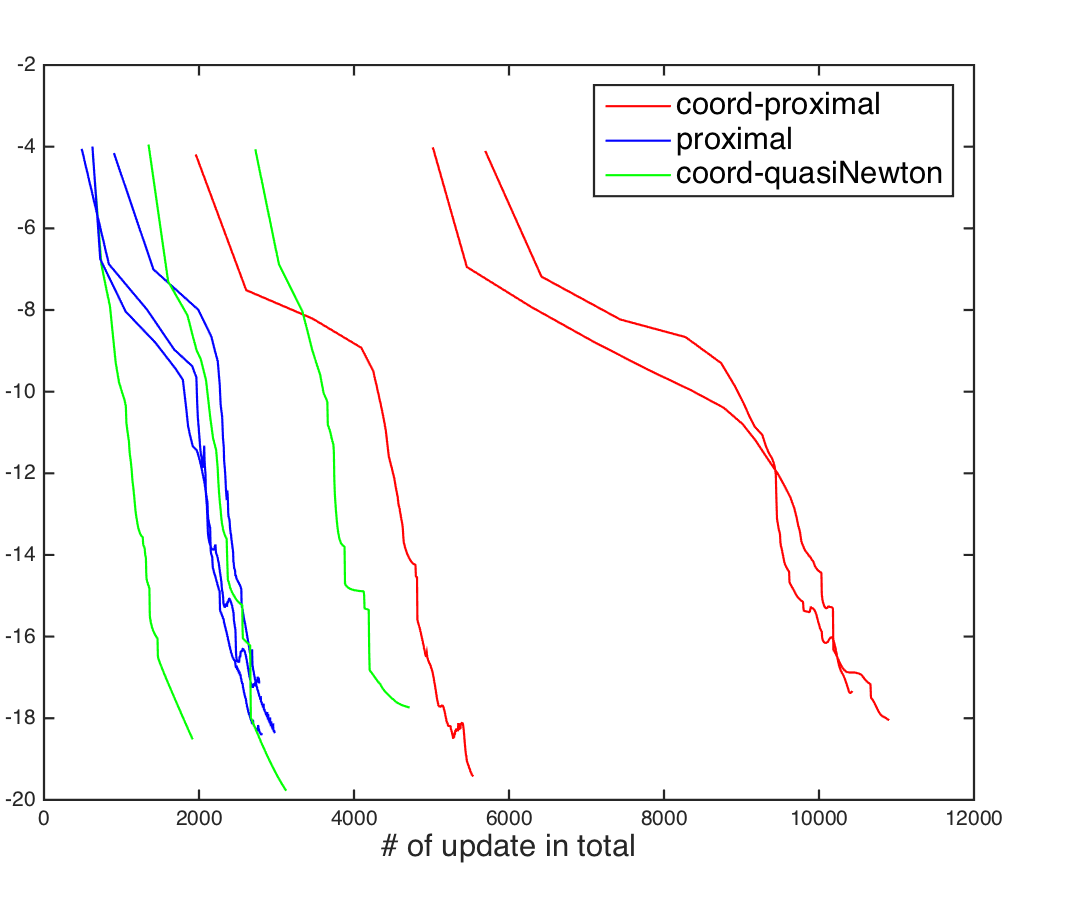
\includegraphics[width=.65\textwidth]{../yanyu_code/plots/sparse_ADMM_feasibility_p30}
  \end{minipage}
  \caption{sparse cFMs (ADMM): The decrease of $\|Z-W\|_F^2$ along ADMM iterations (left to right: SYM, SPARSE, y-axis is $\log(\|Z-W\|_F^2 / p^2)$)}
  \label{fig:feas}
\end{figure}
From the figures we can see, ADMM (proximal) works best almost always. The feasibility curve shows that, as ADMM iteration goes, $Z$ and $W$ gradually match to each other. 

Finally, the performance of ADMM (proximal) is compared to the subgradient method. The performance of ADMM and subgradient method on the same data set are shown in \Cref{fig:subgrad}.
\begin{figure}[ht!]
  \centering
  \begin{minipage}{0.24\textwidth}
    \centering
    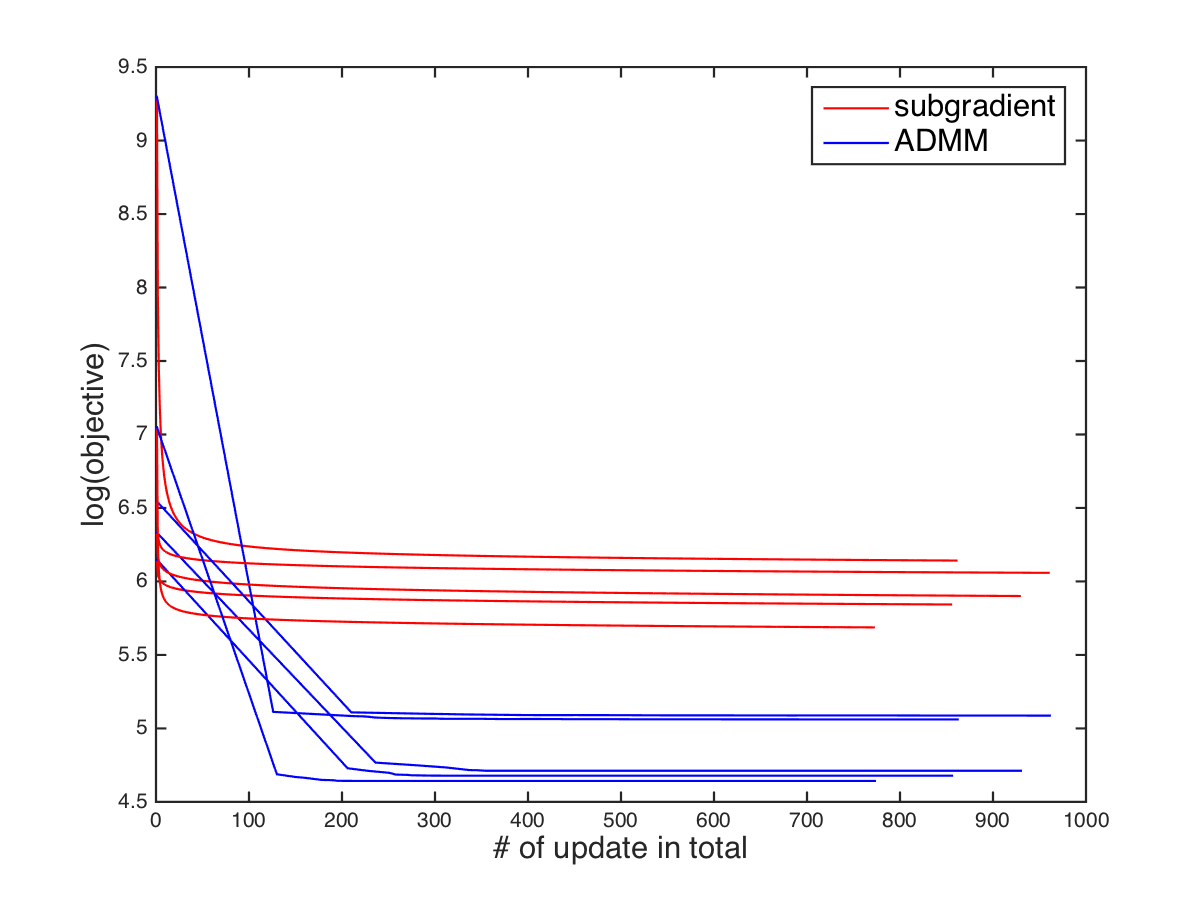
\includegraphics[width=1\textwidth]{../yanyu_code/plots/sym_subgrad_p10}
  \end{minipage}
  \hfill
  \begin{minipage}{0.24\textwidth}
    \centering
    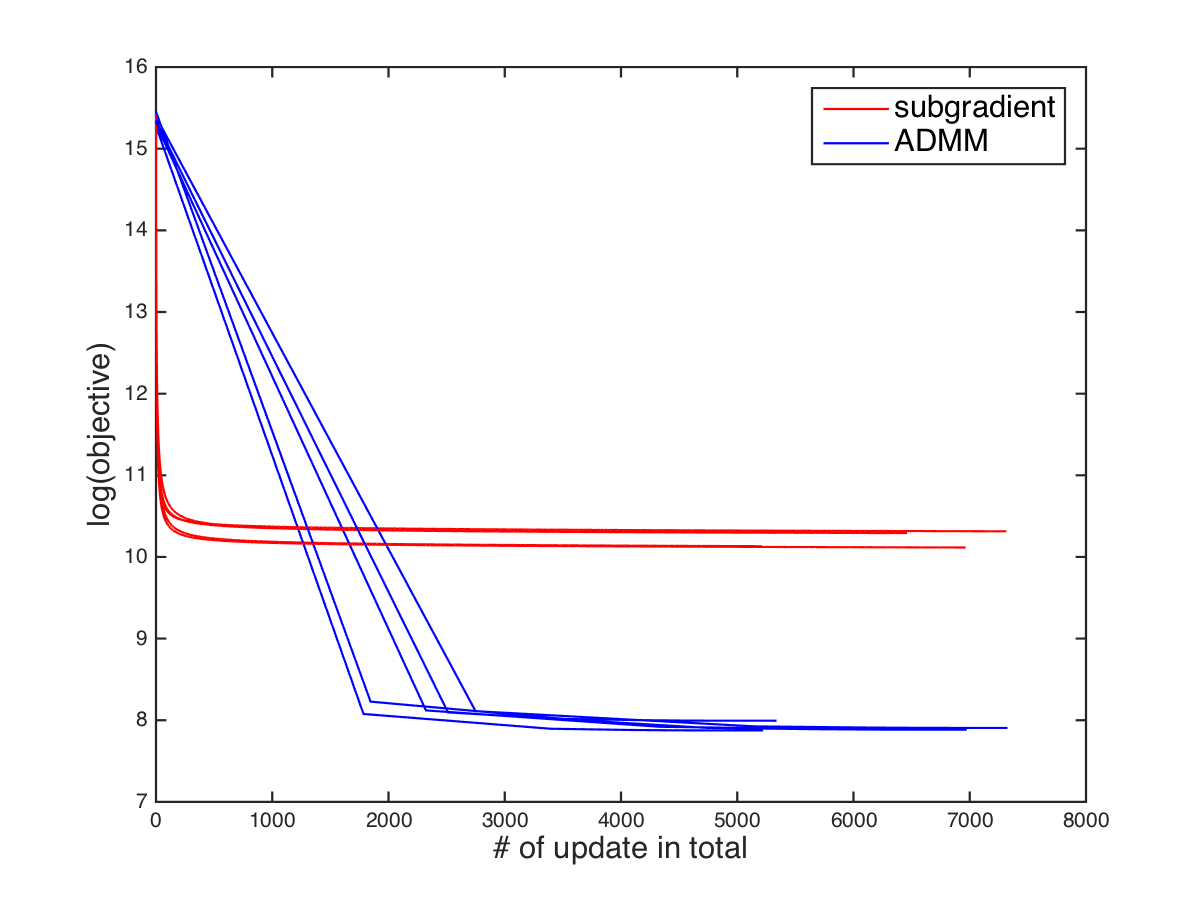
\includegraphics[width=1\textwidth]{../yanyu_code/plots/asym_subgrad_p10}
  \end{minipage}
  \hfill
  \begin{minipage}{0.24\textwidth}
    \centering
    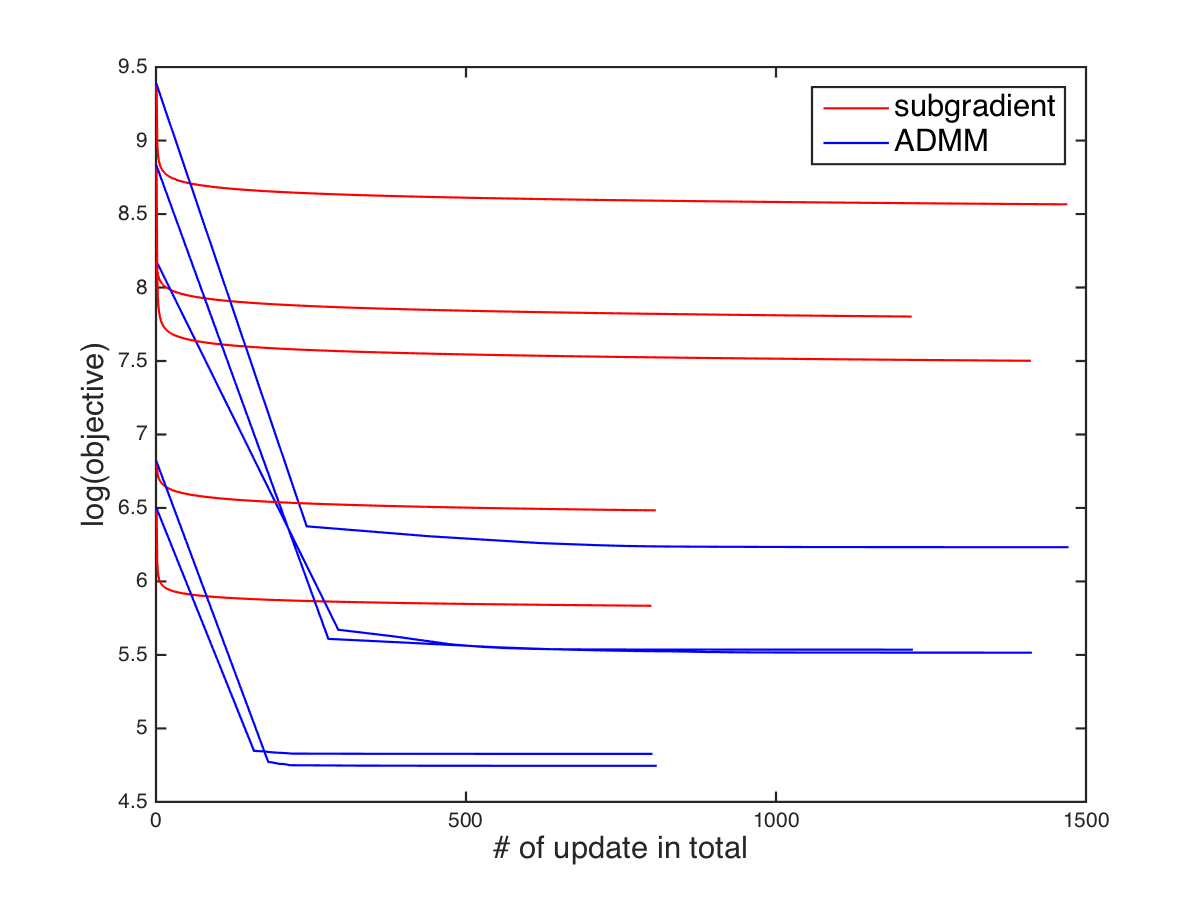
\includegraphics[width=1\textwidth]{../yanyu_code/plots/sparse_subgrad_p10}
  \end{minipage}
  \hfill
  \begin{minipage}{0.24\textwidth}
    \centering
    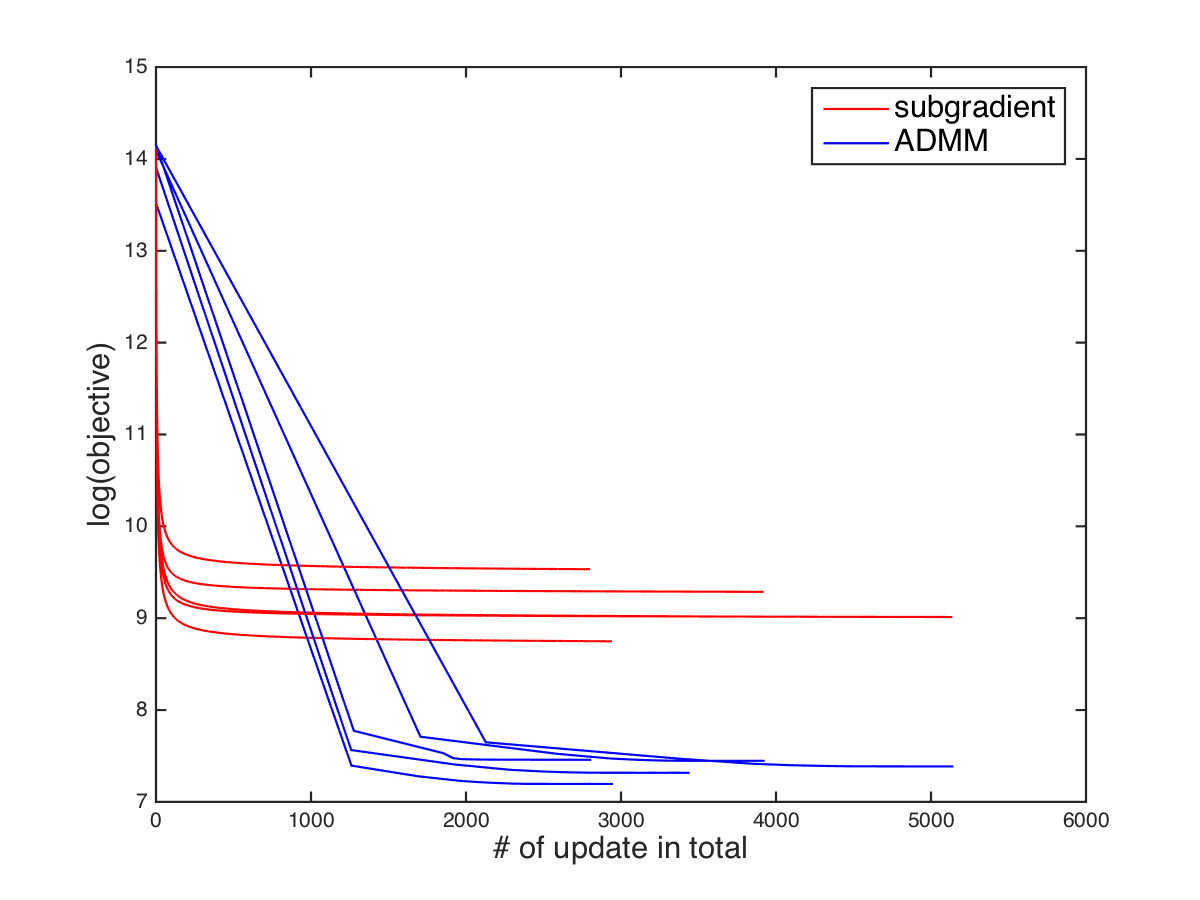
\includegraphics[width=1\textwidth]{../yanyu_code/plots/block_subgrad_p10}
  \end{minipage}
  \caption{ADMM vs subgradient: The convergences of ADMM (proximal) and subgradient on four types of simulated data (left to right: SYM, ASYM, SPARSE, BLOCK)}
  \label{fig:subgrad}
\end{figure}
The comparison is made with the same amount of updades. At the very first step, ADMM needs many steps to converge, but it converges much more quickly than the sub-gradient method.

\subsection{gFMs} \label{sec:result_gfm}

\begin{figure}[htbp]
  \centering
  \begin{minipage}{0.24\textwidth}
    \centering
    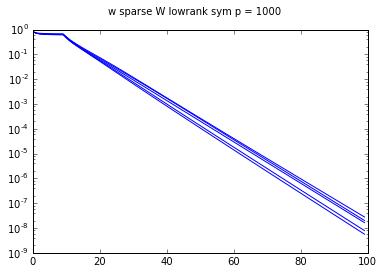
\includegraphics[width=1\textwidth]{gfm_plots/w_sparse_W_lowrank_sym}
  \end{minipage}
  \hfill
  \begin{minipage}{0.24\textwidth}
    \centering
    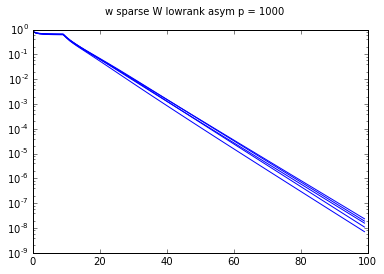
\includegraphics[width=1\textwidth]{gfm_plots/w_sparse_W_lowrank_asym}
  \end{minipage}
  \hfill
  \begin{minipage}{0.24\textwidth}
    \centering
    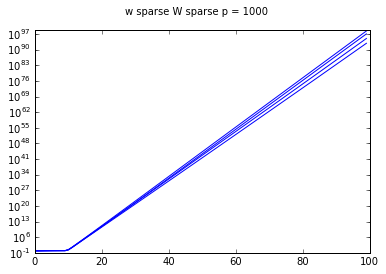
\includegraphics[width=1\textwidth]{gfm_plots/w_sparse_W_lowrank_sparse}
  \end{minipage}
  \hfill
  \begin{minipage}{0.24\textwidth}
    \centering
    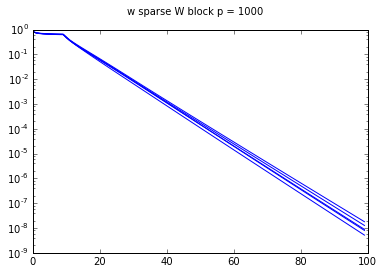
\includegraphics[width=1\textwidth]{gfm_plots/w_sparse_W_block}
  \end{minipage}
  \caption{The convergences of two algorithms on four types of simulated data (top left to bottom right: SYM, ASYM, SPARSE, BLOCK)}
  \label{fig:gfm}
\end{figure}

By running the methods proposed by \cite{generalizedFM_paper} (see \Cref{fig:gfm}), we observed that when gFM is dealing with $W$ that has a sparse structure, the error rate on the training data explodes, probably because its updating through the sequence of estimation does not necessarily require the error change in a descent manner.

Similarly, choosing the rank $k$ of the training data as close to the original rank $k$ is important. As it determines the initialization of $U$ in the algorithm described, estimating $k$ by a large number would almost certainly cause the error rate explodes. The updating rule used in this algorithm is highly sensitive to apriori knowledge about the structure though it can't be easily estimated without certain domain knowledges.

The learning rate, as used to describe the algorithm of gFM, differs from the learning rate we know from algorithms we familiar with from the first order or second order algorithms. Instead, they use learning rate here to denote the degree a single estimation can learn. We tried setting up different learning rate and found that within a certain small window of learning rate, the error rate can decrease linearly with a considerable rate, while with a slightly larger learning rate, linearly increased error rate can be observed.

\section{Discussion}

By replacing greedy coordinate descent algorithms in \cite{convexFM_paper} with proximal gradient descent, we must incorporate SVD, which require much more computing capacity when dealing with large scale matrix. In addition, “one and two stage convergence” and the different convergence rates of each data type still remain mysterious, which leaves a potential interesting theoretical research topic to dive into. We may discover some potential performence improvement space of proximal gradient descent for matrix completion problems.

The motivation to introduce sparsity constraint on $W$ is that in real world application, the interaction between features can be very sparse. For example, in gene expression data, only the genes in the same pathway (regulatory module) have strong coexpression pattern and other coincident correlations should not be considered (they may lead to overfitting). Therefore, in some problem setting, the introduction of element-wise sparsity constraint is potentially useful. Furthermore, within the proposed ADMM, the element-wise sparsity constraint can be easlily extended to other more sophisticated ones, such as group lasso, since the subrountine is equivalent to a regular lasso problem.

Regarding the implementation of ADMM approach, the most time consuming step is to update $w_0, w, W$ since there is no analytical solution. It is the bottleneck for applying the ADMM approach to large-scale problem and it is necessary to develop more sophisticated framework to solve it efficiently, such as second-order method, to use screening techniques to reduce the size of the problem before solving, to construct solution path with warm starts.

For gFMs, generally speaking, its formuation and its associated algorithm bridges the theoretical gap between the matrix sensing problem and the factorization machine. By incorporating different structural information in $W$ for our simulated data, gFM also behaves differently. Specifically, when $W$ is assumed to be sparse, the objective values explodes linearly, while under the same hyper-parameters, linear convergence could be achieved by those other three simulated data. This is probably because sparse $W$ affects the tolerance of higher learning rate of this algorithm, under which the algorithm may fail to converge and the objective values will explode. It is proved that the algorithm they proposed can achieve a linear convergence rate and it is also shown in our experiment. However, we found it to be highly sensitive to hyper-parameters such as learning rate and the rank $k$ before applying this algorithm, which makes it somewhat impractical in a real world setting.


\section*{References}
\small{
\renewcommand{\section}[2]{}%
\bibliography{myref} 
\bibliographystyle{alpha}
}

\end{document}